\documentclass[11pt,titlepage]{article}
\usepackage{fullpage}
\usepackage{amsmath}
\usepackage{amssymb}
\usepackage{color}
\usepackage{graphicx}
\usepackage{subcaption}
\graphicspath{ {images/} }
\usepackage{tikz}
\usetikzlibrary{shapes,arrows,positioning,calc}
\usepackage{float}
\restylefloat{table}
\usepackage{array}
\tikzset{
	block/.style = {draw, fill=white, rectangle, minimum height=3em, minimum width=3em},
	sum/.style = {draw, fill=white, circle, node distance=1cm},
	input/.style = {draw=none},
	output/.style = {draw=none},
	coord/.style = {coordinate}
}

\author{Rane Brown \\ Kate Schneider}
\title{ECEN 4638: Lab X.1P}
\date{\today}

\begin{document}
\maketitle
\tableofcontents
\listoffigures
\newpage

\section{Description}
	The purpose of this lab is to explore the torsion disc system and experimentally collect data that will help in the design of a proportional controller. The torsion disc system consists of a platform with three discs aligned above a driving motor. There are various configurations for the torsion disc system and this lab will use a basic setup described below. 
	\begin{figure}[h!]
			\centering
			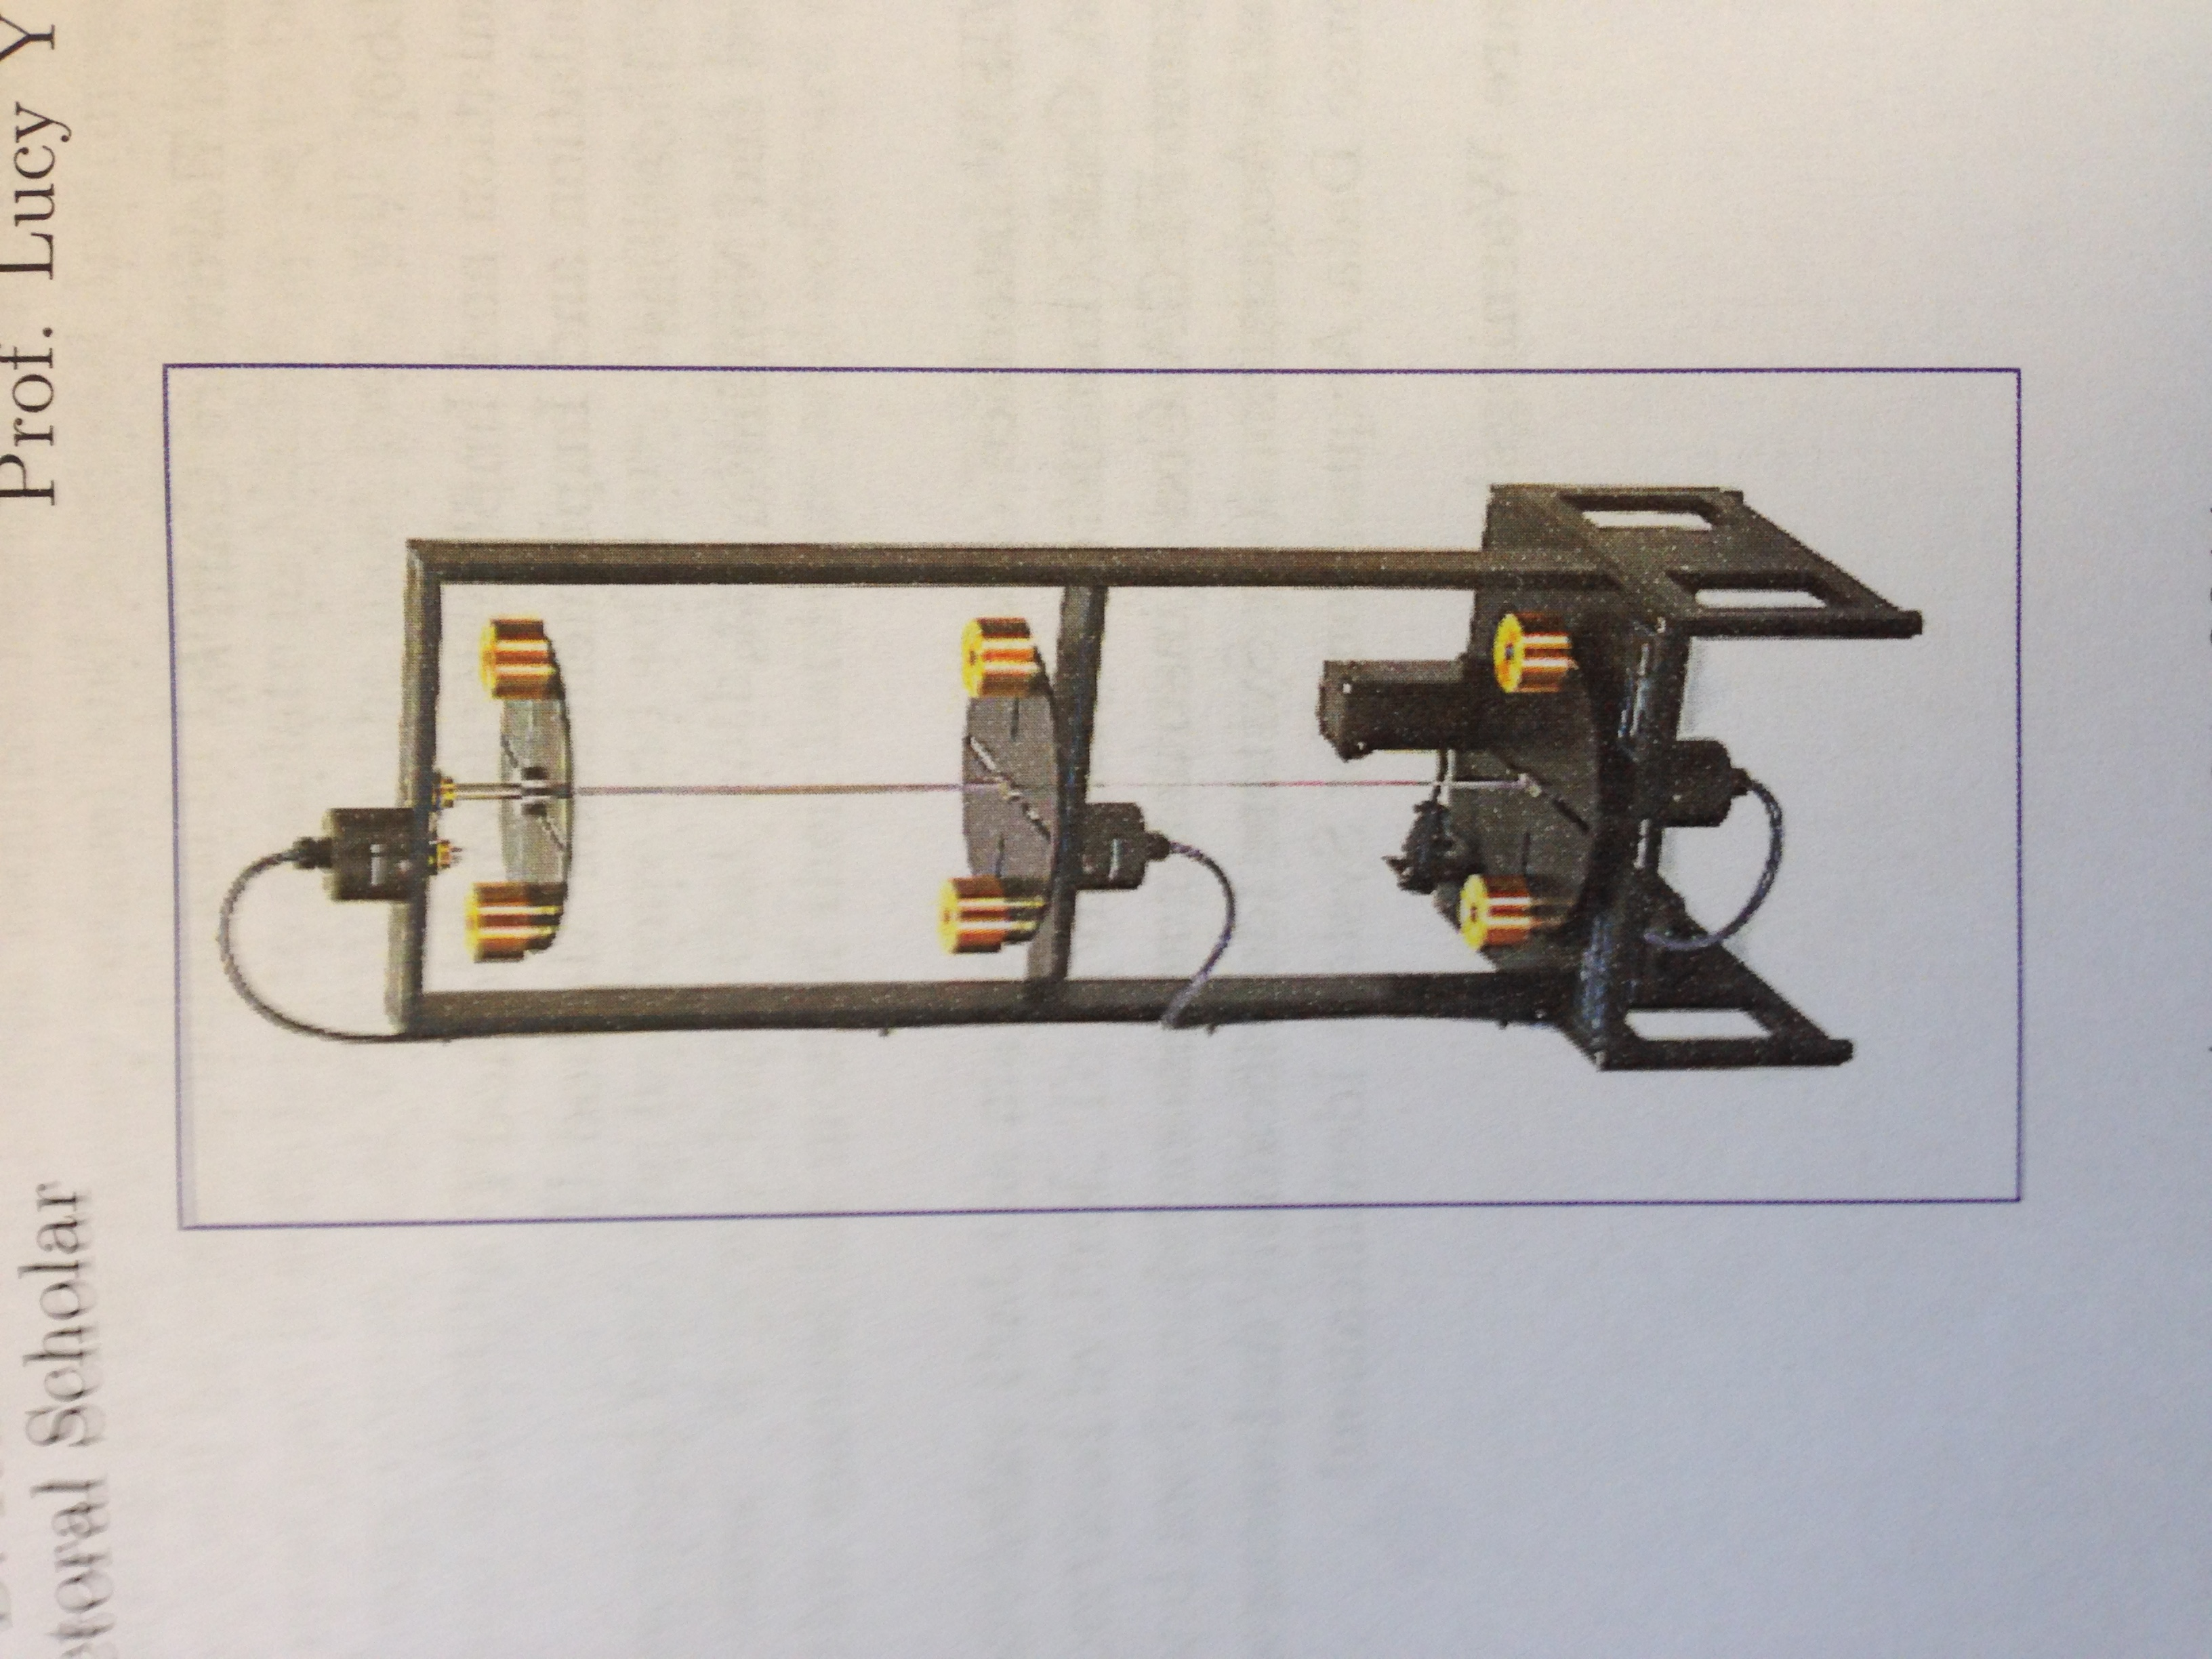
\includegraphics[trim={6cm 0 0 0},clip,angle=-90,origin=c,scale=0.1]{torsionSystem}
			\caption{Torsion Disc System}
			\label{fig:disc_sys}
	\end{figure}

\section{Setup}
	There are three main components that will be necessary for this lab: LabView, Matlab, and the Torsion Disc System. LabView and Matlab do not require any setup as they are installed on all lab computers. On the other hand, the torsion disc system must be configured for proper use. For this experiment the top two discs and any attached weights should be removed. After the weights and discs are removed the system cables can be connected.
	\subsection*{Detailed Steps}
	\begin{enumerate}
		\item loosen allen key screws on all weights attached to the top two discs and remove the weights.
		\item loosen allen key screws on top two discs and detach the discs (each disc is two pieces)
		\item attach all labeled connectors and power lines
	\end{enumerate}

\section{LabView Intro}
	LabView is a high level program that will be used to control the torsion disc system. Data from the system will also be collected using LabView. The general idea is to build a block diagram of the system with appropriate input and output values as well as a configurable controller. In order to understand the operation of LabView it is useful to create a demo system before beginning work on the Torsion Disc system.
	\subsection{Simulation Loop}
		Figure \ref{fig:sim_intro} shows a simulation loop that was created in LabView. Transfer function blocks were used for the vehicle and controller while the reference and disturbance inputs use lookup tables. The output of the system is written to an external file.
		\begin{figure}[h!]
			\centering
			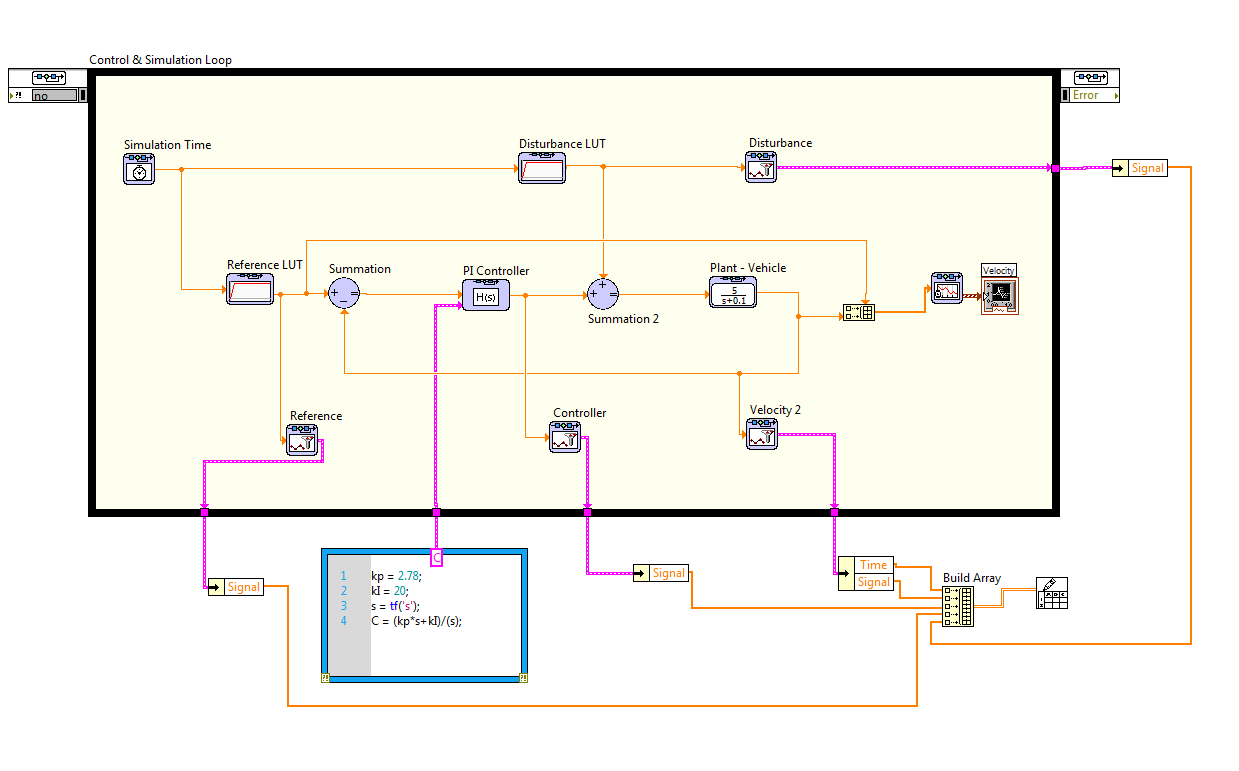
\includegraphics[scale=.5]{labviewIntro}
			\caption{LabView Intro Model}
			\label{fig:sim_intro}
		\end{figure}
	\subsection{Controller Results}
		The created simulation was run with various values of $K_p$ and $K_I$ and the output was observed and recorded. The collected results from the LabView simulations were then taken and compared to the Simulink model used in LabX. As seen in figure \ref{fig:kp1} and figure \ref{fig:kp5KI10}, the results from LabView and simulink are comparable.
		\begin{figure}[h!]
			\centering
			\begin{minipage}{.5\textwidth}
				\centering
				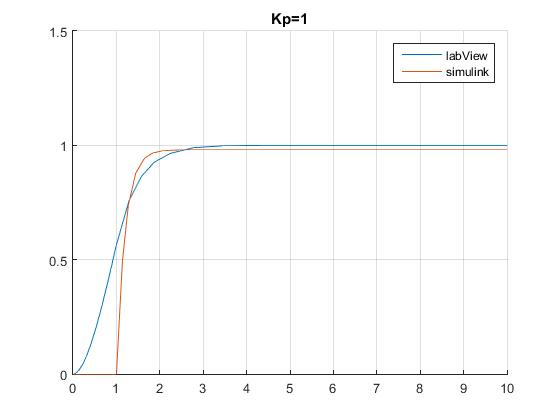
\includegraphics[scale=.4]{Kp1}
				\captionof{figure}{P Controller $K_p=1$}
				\label{fig:kp1}
			\end{minipage}%
			\begin{minipage}{.5\textwidth}
				\centering
				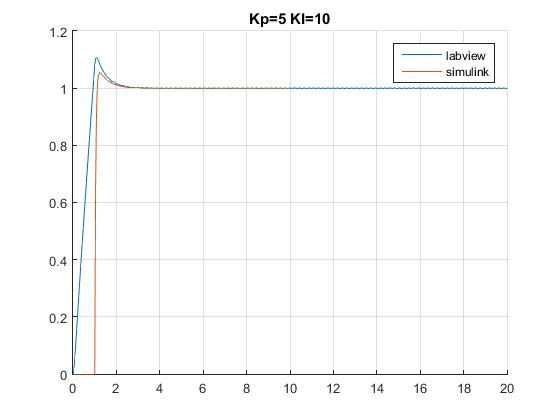
\includegraphics[scale=.4]{Kp5KI10}
				\captionof{figure}{PI Controller $K_p=5$ $K_I=10$}
				\label{fig:kp5KI10}
			\end{minipage}%
		\end{figure}	
	\subsection{Disturbance} 
		As a final experiment a disturbance was introduced to the LabView model that simulates a hill. The $P$ and $P_I$ values were chosen in order to produce a fast response with a small amount of overshoot and a reasonable settle time. In this case, values of $K_I=20$ and $K_I=60$ worked well. The results of this experiment are shown in figure \ref{fig:resp_dist}.
		\begin{figure}[h!]
			\centering
			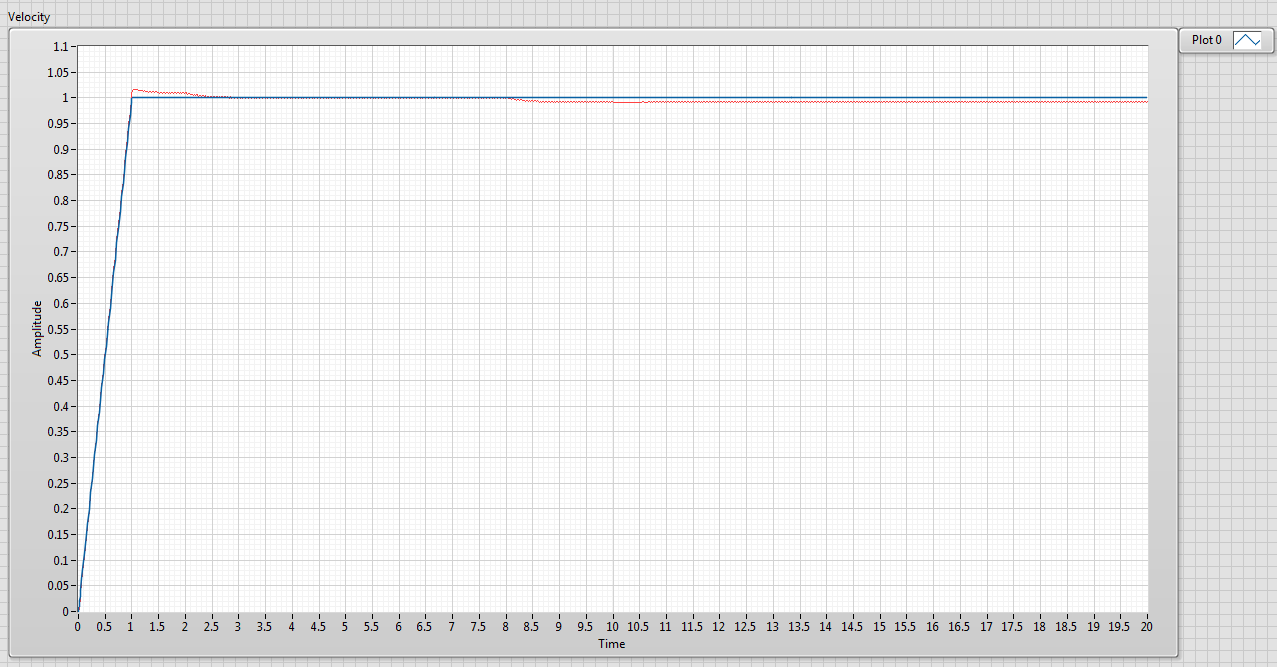
\includegraphics[scale=.4]{disturbance}
			\caption{Response with disturbance}
			\label{fig:resp_dist}
		\end{figure}

\section{Data Collection}
	To create a LTI model for the Torsion Disc system it was necessary to collect data that could be used to estimate system parameters. A LabView model was used to control the system and collect necessary data. The LabView model shown in figure \ref{fig:labview_sys} was provided for this experiment and can be found on the ITLL share drive. Two experiments were conducted to collect the needed data. \emph{NOTE: equations are found in section \ref{sec:LTI}.}
	\begin{figure}[h!]
			\centering
			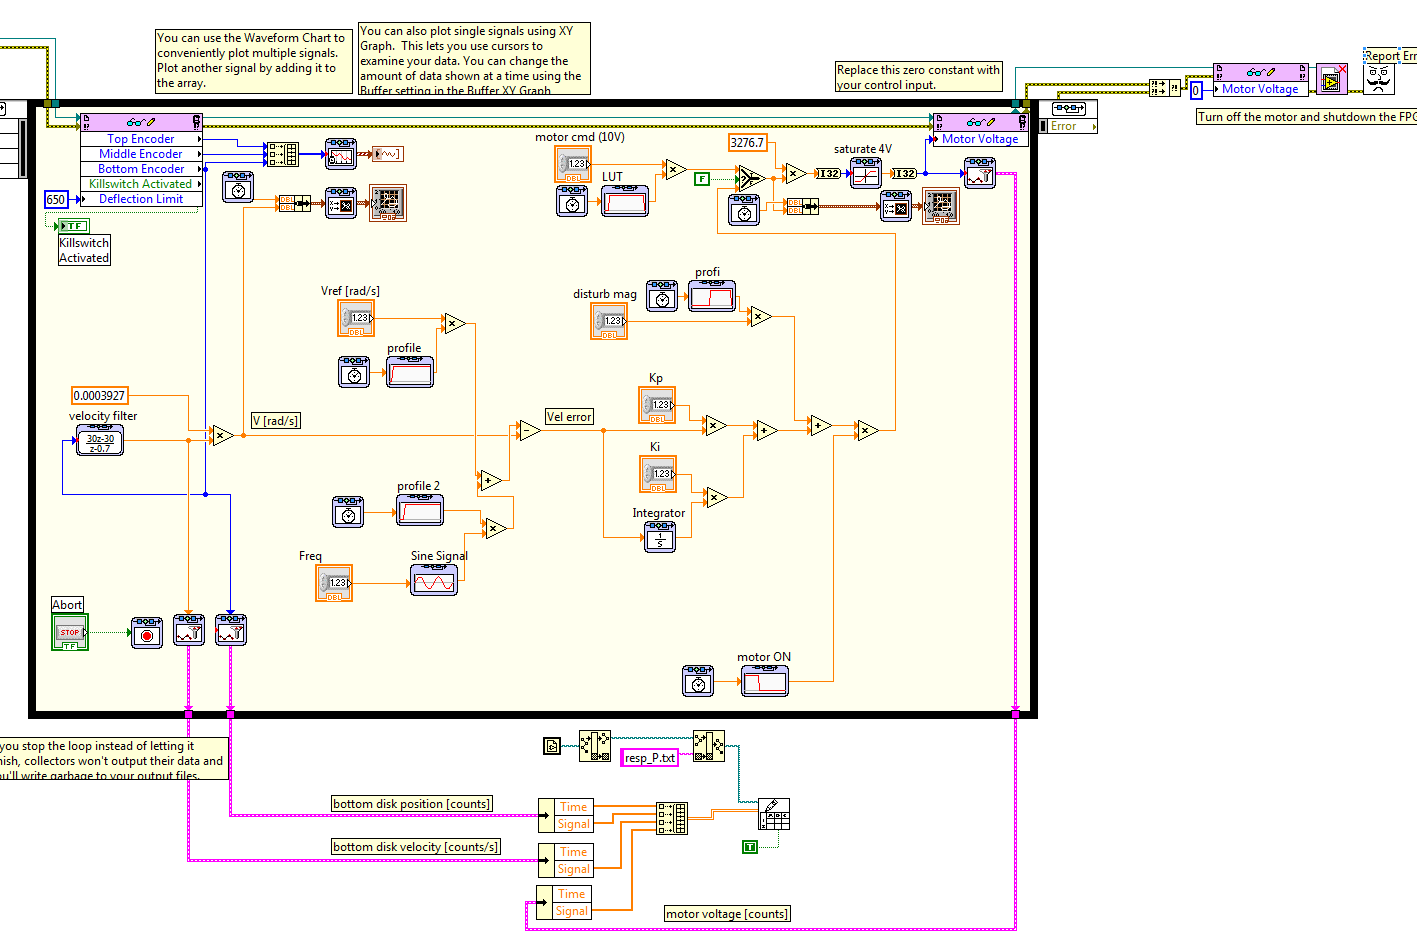
\includegraphics[trim={0 0 10cm 0},clip,scale=0.4]{labviewModel}
			\caption{LabView Control System}
			\label{fig:labview_sys}
	\end{figure}
	\subsection{No motor voltage}
		The first experiment was conducted with no power connected to the Torsion Disc motor. This was done in order to eliminate some of the parameters from the LTI model in order to estimate the value of $c$. Data was collected for three different weight positions as shown in table \ref{table:weight_pos}. Each weight position gives a different inertia value for the system. The data is collected by first selecting a weight position and then manually spinning the disc by hand. \emph{If only 2 weights are used they must be located along the hub split line.}
	\subsection*{Steps}
		\begin{enumerate}
			\item set the weights to a desired radius on the lower disc
			\item make sure the bolts holding the weights are firmly tightened
			\item begin data collection in LabView
			\item manually spin the disc and allow it to come to a stop
			\item data is saved as a text file
			\item change filename to reflect the weight position
		\end{enumerate}
			\textcolor{red}{Verify weight radius, add inertias}
		\begin{table}[h!]
			\centering
			\begin{tabular}{|m{4cm}|m{3cm}|m{3cm}|} 
				\hline
				Number of weights & Radius & Inertia $J$ \\ 
				\hline
				4 & 9 cm & val \\
				\hline
				4 & 7.5 cm & val\\
				\hline
				2 & 4 cm & val \\
				\hline
			\end{tabular}
			\caption{Weights and Position} \label{table:weight_pos}
		\end{table}
	\subsection{Powered Torsion Disc System}
	The second data collection experiment was conducted with the power connected to the Torsion Disc system. In this case the values of various system parameters are adjusted in LabView while the weights remain in the same position. The collected data is then used to create a proportional controller.
	\subsection*{Steps}
		\begin{enumerate}
			\item set reference speed to 3.14 rad/sec
			\item set disturbance to 0
			\item set $K_p$ to 1
			\item adjust experiment length to 12 seconds in order to collect data as the system comes to a stop
			\item \textbf{Ensure there is someone with their finger on the power of button in case the system goes unstable}
			\item turn the power on
			\item press the run button in LabView, data is saved as a text file
			\item rename file to reflect parameter values
			\item repeat for the values listed in below table
		\end{enumerate}
		\textcolor{red}{add table showing values we collected data for}

\section{LTI Model} \label{sec:LTI}
	The Torsion Disc system can be modeled as an LTI system with the below equation.
	\begin{equation} \label{eq:lti}
		J\dot{\omega}+c\omega=k_hu
	\end{equation}
	Where $J=\mbox{ total system inertia}$, $\omega=\mbox{ velocity rad/sec}$, $c=\mbox{ system drag}$, $k_h=\mbox{ hardware gain}$, $u=\mbox{ reference}$.

	\subsection{Estimating model values}
	Using equation \ref{eq:lti} and the collected data the value of $c$ can be estimated.

\section{Proportional Controller Design}

\end{document}